\documentclass[a4paper,11pt]{article}
\usepackage{booktabs} % Provides professional-quality horizontal rules
\usepackage{float} % Required for [H] placement
\usepackage{tikz}
\usepackage{hyperref}
\usepackage[bottom=1.5in]{geometry}

\hypersetup{
    colorlinks=true,    % True removes the default red/green border boxes
    linkcolor=blue,     % Colors internal links (like the TOC) blue
    urlcolor=cyan       % Colors external URLs cyan
}

\newcommand{\newpagex}{
    \newpage
    \vspace*{-7\baselineskip} % Pulls text up by one line
}

\author{Hectron} 

\title{Minimum Substring}

\begin{document}

% generates the title
\maketitle

% insert the table of contents
\tableofcontents

% seperate body and table of contents 
\newpagex
    \noindent

\section{Description}
    
We can scramble a string s to get a string t using the following algorithm:


    \begin{itemize}
        \item If the length of the string is 1, stop.
        \item  If the length of the string is > 1, do the following:
        \begin{itemize} 
            \item Split the string into two non-empty substrings at a random index, i.e., if the string is s, divide it to x and y where s = x + y.
            \item Randomly decide to swap the two substrings or to keep them in the same order. i.e., after this step, s may become s = x + y or s = y + x.
            \item Apply step 1 recursively on each of the two substrings x and y.
        \end{itemize}
    \end{itemize}
    Given two strings s1 and s2 of the same length, return true if s2 is a scrambled string of s1, otherwise, return 



    \begin{itemize}
    \item \textbf{Input:} \newline \textmd{s1 = ``great''} \newline \textmd{s2 = ``rgeat''}
    \item \textbf{Output}: \newline  \textmd{``true''}
    \end{itemize}

\section{Function/Method Declaration} 
\footnotesize
\begin{verbatim}
class Solution {
public:
    bool isScramble(std::string s1, std::string s2) {
        /*
            s1 - string pattern 
            s2 - string target. Scrambling s1 must follow this target pattern structure
        */
    }
}
\end{verbatim}

\section{How to solve}
\textcolor{blue}{s1 - data } \\
\textcolor{red}{s2 - target rule } 
    


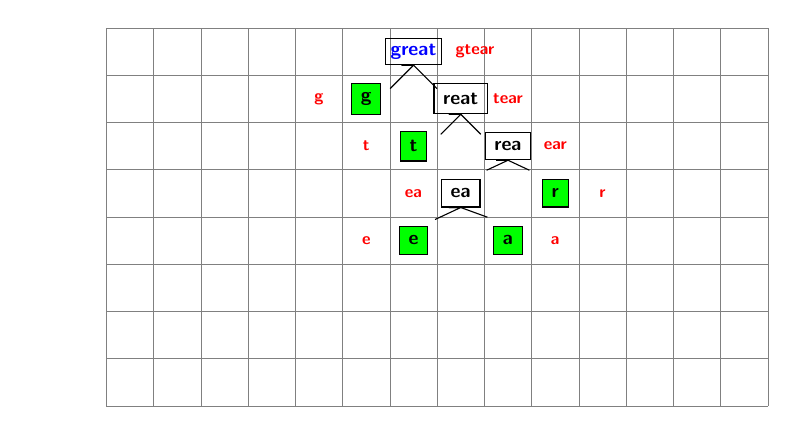
\begin{tikzpicture}[node distance=1.0cm , trim left=-1cm, scale=0.6]

    \draw[help lines, opacity=1] (0,0) grid (14,8 );

    % \node (p)  at ( -1.0, 7.5) [draw, font=\fontsize{7}{9}\selectfont\sffamily\bfseries] {sequence};
    % \node (p2)  at ( -1.0, 6.5) [draw, font=\fontsize{7}{9}\selectfont\sffamily\bfseries] {accNodes0};
    % \node (p3)  at ( -1.0, 5.5) [draw, font=\fontsize{7}{9}\selectfont\sffamily\bfseries] {accNodes1};
    % \node (p3)  at ( -1.0, 4.5) [draw, font=\fontsize{7}{9}\selectfont\sffamily\bfseries] {accNodes2};
    % \node (p4)  at ( -1.0, 3.5) [draw, font=\fontsize{7}{9}\selectfont\sffamily\bfseries] {accNodes3};
    % \node (p5)  at ( -1.0, 2.5) [draw, font=\fontsize{7}{9}\selectfont\sffamily\bfseries] {accNodes4};

    \node (seq0)  at ( 6.5, 7.5 )[text=blue,inner sep=2pt, draw, font=\fontsize{7}{9}\selectfont\sffamily\bfseries] {great};
    \node ()  at ( 7.8, 7.5 )[text=red, font=\fontsize{6}{5}\selectfont\sffamily\bfseries] {gtear};

    % \node (seq0)  at ( 0.5, 7.5) \drawnode{} {A};
    \draw[-] (seq0.south) -- ++(-0.25, 0 ) -- (seq0.south) -- ++(-45 : 0.7cm ) ;
    
    \draw[-] (seq0.south) -- ++(-0.25, 0 ) -- (seq0.south) -- ++( 225 : 0.7cm ) ;

    \node (seq1)  at ( 5.5, 6.5) [fill=green, draw, font=\fontsize{7}{9}\selectfont\sffamily\bfseries] {g};
    \node ()  at ( 4.5, 6.5 )[text=red, font=\fontsize{6}{5}\selectfont\sffamily\bfseries] {g};

    \node (seq2)  at ( 7.5, 6.5) [draw, font=\fontsize{7}{9}\selectfont\sffamily\bfseries] {reat};
    \node ()  at ( 8.5, 6.5 )[text=red,font=\fontsize{6}{5}\selectfont\sffamily\bfseries] {tear};

    \draw[-] (seq2.south) -- ++(-0.25, 0 )  -- (seq2.south) -- ++(-45 : 0.6cm ) ;
    \draw[-] (seq2.south) -- ++(-0.25, 0 )  -- (seq2.south) -- ++(225 : 0.6cm ) ;

    \node (seq3)  at ( 6.5, 5.5) [fill=green,draw, font=\fontsize{7}{9}\selectfont\sffamily\bfseries] {t};
    \node ()  at ( 5.5, 5.5 )[text=red,font=\fontsize{6}{5}\selectfont\sffamily\bfseries] {t};

    \node (seq4)  at ( 8.5, 5.5) [draw, font=\fontsize{7}{9}\selectfont\sffamily\bfseries] {rea};
    \node ()  at ( 9.5, 5.5 )[text=red,font=\fontsize{6}{5}\selectfont\sffamily\bfseries] {ear};
    
    \draw[-] (seq4.south) -- ++(-0.25, 0 )  -- (seq4.south) -- ++(-25 : 0.5cm ) ;
    \draw[-] (seq4.south) -- ++(-0.25, 0 )  -- (seq4.south) -- ++(205 : 0.5cm ) ;

    \node (seq5)  at ( 7.5, 4.5) [draw, font=\fontsize{7}{9}\selectfont\sffamily\bfseries] {ea};
    \node ()  at ( 6.5, 4.5 )[text=red,font=\fontsize{6}{5}\selectfont\sffamily\bfseries] {ea};
    \node (seq6)  at ( 9.5, 4.5) [fill=green,draw, font=\fontsize{7}{9}\selectfont\sffamily\bfseries] {r};
    \node ()  at ( 10.5, 4.5 )[text=red,font=\fontsize{6}{5}\selectfont\sffamily\bfseries] {r};

    \draw[-] (seq5.south) -- ++(-0.25, 0 )  -- (seq5.south) -- ++(-20 : 0.6cm ) ;
    \draw[-] (seq5.south) -- ++(-0.25, 0 )  -- (seq5.south) -- ++(-155 : 0.6cm ) ;

    \node (seq7)  at ( 6.5, 3.5) [fill=green,draw, font=\fontsize{7}{9}\selectfont\sffamily\bfseries] {e};
    \node ()  at ( 5.5, 3.5 )[text=red,font=\fontsize{6}{5}\selectfont\sffamily\bfseries] {e};
    \node (seq8)  at ( 8.5, 3.5) [fill=green,draw, font=\fontsize{7}{9}\selectfont\sffamily\bfseries] {a};
    \node ()  at ( 9.5, 3.5 )[text=red,font=\fontsize{6}{5}\selectfont\sffamily\bfseries] {a};

    % \node (seq2)  at ( 2.5, 7.5) [draw, font=\fontsize{7}{9}\selectfont\sffamily\bfseries] {O};
    % % \draw[-] (seq2.south) -- ++(-0.25, 0 )  -- (seq2.south) -- ++(225 : 0.75cm ) ;
    % % \draw[-] (seq2.south) -- ++(-0.25, 0 )  -- (seq2.south) -- ++(-45 : 0.75cm ) ;

    % \node (seq3)  at ( 3.5, 7.5) [draw, font=\fontsize{7}{9}\selectfont\sffamily\bfseries] {B};
   

\end{tikzpicture}


    \begin{figure}[htbp]
            \vspace{-15pt} % Essential anchor to force top alignment
        % \caption{Search for minimum substring example.}
            \caption{Branch network created by solver.}
        \end{figure}
\end{document}

